\section*{Abstract}
		This overview presents the complete T0 Theory series consisting of 8 fundamental documents, which represent a geometric reformulation of physics. Based on a single parameter $\xi = \frac{4}{3} \times 10^{-4}$, together with fixed rational structural choices, fundamental constants, particle masses, and physical phenomena from quantum mechanics to cosmology are described within one framework; SI anchors such as $E_0$, $m_e$ or $v$ serve for conversion, not for derivation. Many values are matched to about 1\,\%; because the ladder parameters $r_i$, $p_i$ are set and one anchor provides the connection to SI, these agreements are not independent evidence. The series deliberately leaves the cosmic sector ($H_0$, $\Lambda$, dark energy) aside, because the Standard Model does not derive it either; the cosmological statements are speculative. The theory offers testable predictions for future experiments.

	

	\section{Document Series: Systematic Structure}
	
	\subsection{Hierarchical Structure of the 8 Documents}
	
	The T0 document series follows a logical progression from fundamental principles to specific applications:
	
	\begin{center}
		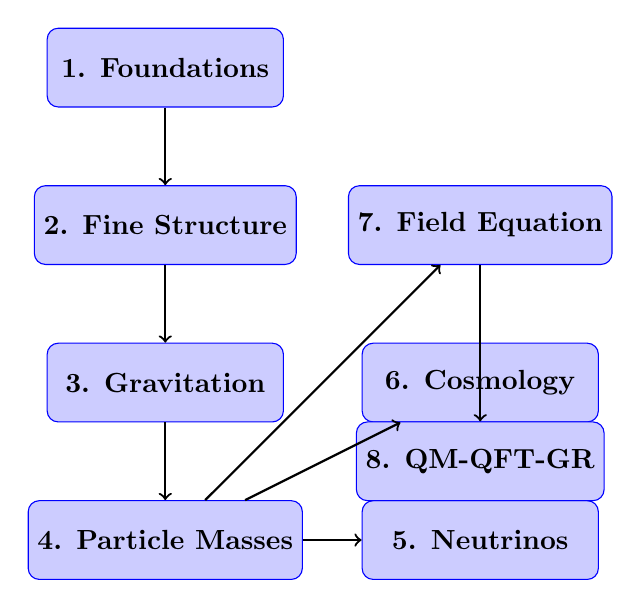
\begin{tikzpicture}[node distance=2cm]
			\tikzstyle{doc} = [rectangle, rounded corners, minimum width=3cm, minimum height=1cm, text centered, draw=blue, fill=blue!20]
			\tikzstyle{arrow} = [thick,->]
			
			\node [doc] (doc1) {\textbf{1. Foundations}};
			\node [doc, below of=doc1] (doc2) {\textbf{2. Fine Structure}};
			\node [doc, below of=doc2] (doc3) {\textbf{3. Gravitation}};
			\node [doc, below of=doc3] (doc4) {\textbf{4. Particle Masses}};
			\node [doc, right of=doc4, xshift=2cm] (doc5) {\textbf{5. Neutrinos}};
			\node [doc, above of=doc5] (doc6) {\textbf{6. Cosmology}};
			\node [doc, above of=doc6] (doc7) {\textbf{7. Field Equation}};
			\node [doc, below of=doc7, yshift=-1cm] (doc8) {\textbf{8. QM-QFT-GR}};
			
			\draw [arrow] (doc1) -- (doc2);
			\draw [arrow] (doc2) -- (doc3);
			\draw [arrow] (doc3) -- (doc4);
			\draw [arrow] (doc4) -- (doc5);
			\draw [arrow] (doc4) -- (doc6);
			\draw [arrow] (doc4) -- (doc7);
			\draw [arrow] (doc7) -- (doc8);
		\end{tikzpicture}
	\end{center}
	
	\section{Document 1: 003\_T0\_Grundlagen\_v1\_En.pdf}
	
	\begin{documentbox}
		\textbf{Subtitle:} The Geometric Foundations of Physics
		
		\textbf{Core Contents:}
		\begin{itemize}
			\item \textbf{Fundamental Parameter:} $\xi = \frac{4}{3} \times 10^{-4}$ as a geometric constant
			\item \textbf{Time-Mass Duality:} $T \cdot m = 1$ in natural units
			\item \textbf{Fractal Spacetime Structure:} $D_f^{\text{eff}} \approx 2.973$ and $K_{\text{frak}} \approx 0.987$
			\item \textbf{Interpretation Levels:} Harmonic, geometric, field-theoretic
			\item \textbf{Universal Formula Structure:} Template for all T0 relations
		\end{itemize}
		
		\textbf{Fundamental Insights:}
		\begin{itemize}
			\item Tetrahedral packing as the fundamental spatial structure
			\item Quantum field-theoretic derivation of $10^{-4}$
			\item Characteristic energy scales: $E_0 = 7.398$ MeV
			\item Philosophical implications of geometric physics
		\end{itemize}
		
		\textbf{Status:} Theoretical foundation - fully established
	\end{documentbox}
	
	\section{Document 2: 011\_T0\_Feinstruktur\_En.pdf}
	
	\begin{documentbox}
		\textbf{Subtitle:} Derivation of $\alpha$ from geometric principles
		
		\textbf{Central Formula:}
		\begin{equation}
			\boxed{\alpha = \xi \cdot \left(\frac{E_0}{1\,\text{MeV}}\right)^2}
		\end{equation}
		
		\textbf{Key Results:}
		\begin{itemize}
			\item \textbf{T0 Value:} $\alpha^{-1} = 137.04$
			\item \textbf{Experiment:} $\alpha^{-1} = 137.036$
			\item \textbf{Deviation:} 0.003\%
			\item \textbf{Assessment:} The agreement is a property of the anchor $E_0$, which provides the only connection to the SI; it is not an independent prediction.
		\end{itemize}
		
		\textbf{Theoretical Innovations:}
		\begin{itemize}
			\item Characteristic energy $E_0 = \sqrt{m_e \cdot m_\mu/K_{\text{frak}}}$ (bare $\sqrt{m_e m_\mu}$, R72)
			\item Logarithmic symmetry of lepton masses
			\item Fundamental dependence $\alpha = \xi E_0^2$ with $E_0 = \sqrt{m_e m_\mu/K_{\text{frak}}}$
			\item Why numerical ratios must not be canceled
		\end{itemize}
		
		\textbf{Status:} $\alpha = \xi E_0^2$ as a relation via the anchor $E_0$
	\end{documentbox}
	
	\section{Document 3: 012\_T0\_Gravitationskonstante\_En.pdf}
	
	\begin{documentbox}
		\textbf{Subtitle:} Systematic derivation of $G$ from geometric principles
		
		\textbf{Complete Formula:}
		\begin{equation}
			\boxed{G_{\text{SI}} = \frac{\xi^2}{4 m_e} \times C_{\text{conv}} \times K_{\text{frak}}}
		\end{equation}
		
		\textbf{Conversion Factors:}
		\begin{itemize}
			\item \textbf{Dimensional Correction:} $C_1 = 1/E_{\text{char}} = 3.472 \times 10^{-2}$ with $E_{\text{char}} = 28.8$ (Doc.~012); $C_1$ does not appear in the boxed formula above, which holds without $C_1$
			\item \textbf{SI Conversion:} $C_{\text{conv}} = 7.783 \times 10^{-3}$
			\item \textbf{Fractal Correction:} $K_{\text{frak}} = 0.986$
		\end{itemize}
		
		\textbf{Experimental Verification:}
		\begin{itemize}
			\item \textbf{T0 Prediction:} $G = 6.6745 \times 10^{-11}$ m³/(kg·s²)
			\item \textbf{CODATA 2018:} $G = 6.67430 \times 10^{-11}$ m³/(kg·s²)
			\item \textbf{Deviation:} +0.003\%
		\end{itemize}
		
		The boxed formula with the stated factors gives $6.6745\times10^{-11}$. $C_{\text{conv}}$ is the SI conversion of the single-anchor chain (Doc.~383); its numerical value $7.783\times10^{-3}$ additionally contains the small residual of this chain (chain value $7.58\times10^{-3}$). The form of $G$ and its order of magnitude follow from $\xi$ and the one anchor (numerically checked in Doc.~383); with the anchor $m_e$, $G$ lies at $-2.6\,\%$, with $v$ at $-0.46\,\%$. The agreement to $0.003\,\%$ arises only with this residual and does not count as an independent precision result.
		
		\textbf{Physical Meaning:} Gravity as geometric spacetime-matter coupling
		
		\textbf{Status:} Form and order of magnitude from $\xi$ and one anchor; the CODATA agreement is not an independent precision result
	\end{documentbox}
	
	\section{Document 4: 006\_T0\_Teilchenmassen\_En.pdf}
	
	\begin{documentbox}
		\textbf{Subtitle:} Fermion masses from the ladder $m_i = r_i\,\xi^{p_i}\,v$
		
		\textbf{Two Equivalent Methods:}
		\begin{enumerate}
			\item \textbf{Direct Method:} $m_i = 1/(\xi f_i)$, linked to the Yukawa method via $f_i = 1/(r_i\,\xi^{p_i+1}\,v)$; the agreement of both methods holds by construction
			\item \textbf{Extended Yukawa:} $m_i = y_i \times v$ with $y_i = r_i \times \xi^{p_i}$
		\end{enumerate}
		
		\textbf{Quantum Number System:} Rational quantum numbers $(r_i, p_i)$ as fixed structural choices; $v$ serves as conversion anchor
		
		\textbf{Comparison with Experiment:} For charged leptons and quarks the average deviation is below 1\,\%. Because $r_i$ and $p_i$ are set and adjusted to the measured values, these agreements are identities of the ladder and not evidence in their own right; the mass ratios follow from the ladder to a few digits. Neutrino masses are not calculated in Doc.~006 (Doc.~340 is authoritative); boson masses are treated in Doc.~372 and~373.
		
		\textbf{Reduction:} The free mass parameters of the Standard Model are traced back to $\xi$ and the set rational quantum numbers $(r_i, p_i)$; no continuously adjustable parameter remains.
		
		\textbf{Status:} Ladder structure with set quantum numbers and one anchor
	\end{documentbox}
	
	\section{Document 5: 007\_T0\_Neutrinos\_En.pdf}
	
	\begin{documentbox}
		\textbf{Subtitle:} The Photon Analogy and Geometric Oscillations
		
		\textbf{Approach:}
		\begin{itemize}
			\item \textbf{Photon Analogy:} Neutrinos as 'damped photons'
			\item \textbf{Double $\xi$-Suppression:} base value $m_\nu = \frac{\xi^2}{2} \times m_e = 4.54$ meV
			\item \textbf{Geometric Oscillations:} Phases instead of mass differences
		\end{itemize}
		
		\textbf{Experimental Context:}
		\begin{itemize}
			\item \textbf{Spectrum:} A spectrum that is (nearly) uniform for all flavors, with $\Sigma m_\nu \approx 13.6$ meV, is excluded, because the measured mass differences require $\Sigma m_\nu \geq 59$ meV.
			\item \textbf{Velocity:} An energy-independent difference $v_\nu = c(1 - \xi^2/2)$ does not hold, because $\xi^2/2$ is the mass ratio $m_\nu/m_e$.
			\item \textbf{Authoritative:} For neutrinos, Doc.~340 is authoritative; there the base value $4.54$ meV reappears as the lightest mass $m_{\nu_1}$.
		\end{itemize}
		
		\textbf{Status:} Speculative; the spectrum of Doc.~007 is excluded by the oscillation data, Doc.~340 is authoritative
	\end{documentbox}
	
	\section{Document 6: 025\_T0\_Kosmologie\_En.pdf}
	
	\begin{documentbox}
		\textbf{Subtitle:} Static Universe and $\xi$-Field Manifestations
		
		\textbf{Revolutionary Cosmology:}
		\begin{itemize}
			\item \textbf{Static Universe:} No Big Bang, eternally existing
			\item \textbf{Time-Energy Duality:} No singular beginning, because $T\cdot E = 1$ with the lower time bound $T_0 = \xi\,t_P$ bounds the energy from above and the torus has no boundary (Doc.~306)
			\item \textbf{CMB from $\xi$-Field:} Not from z=1100 decoupling
		\end{itemize}
		
		\textbf{Casimir-CMB Connection:}
		\begin{itemize}
			\item \textbf{Characteristic Length:} $L_\xi = 100$ $\mu$m
			\item \textbf{Ratio at $L_\xi$:} $|\rho_{\text{Casimir}}|/\rho_{\text{CMB}} = 308$ -- an identity, not a measurement result, because $L_\xi$ itself is determined from the measured CMB energy density and $\xi$; a comparison value of $312$ is the same formula with a rounded $L_\xi$. The connection is a statement about scales (speculative).
			\item \textbf{In depth:} Doc.~279 -- Casimir-CMB-H$_0$ connection formula, $L_\xi H_0/c = K_{\text{geo}}\,(m_e c^2/k_B T_{\text{CMB}})\,\xi^{41/4}$.
		\end{itemize}
		
		\textbf{Alternative Redshift (static, achromatic):}
		\begin{equation}
			1+z = e^{\xi x}, \qquad z \approx \xi \cdot x
		\end{equation}
		The fractal path lengthening is purely geometric and stretches all
		wavelengths by the same factor; the redshift is \emph{achromatic}
		(finite-element simulation). The length scale of $x$ does not follow from $\xi$
		alone but is calibrated via the measured $H_0$. In depth:
		Doc.~280 (z$\to$time as a $\Lambda$CDM translation, cosmological degeneracy
		Doc.~267, $z_*\approx 875$ as a T$^4$ lattice resonance).
		
		\textbf{Cosmological Problems (speculative):}
		\begin{itemize}
			\item Horizon problem, flatness problem, monopole problem, age problem
			\item $H_0$ and $\Lambda$ do not follow from $\xi$ alone: the scale of the redshift is calibrated via the measured $H_0$. Hubble tension and dark energy are therefore not regarded as solved; the cosmic sector is deliberately left aside, because the Standard Model does not derive it either.
		\end{itemize}
		
		\textbf{Status:} Testable hypotheses - speculative alternative, cosmic sector calibrated
	\end{documentbox}
	
	\section{Document 7: 019\_T0\_lagrndian\_En.pdf}
	
	\begin{documentbox}
		\textbf{Subtitle:} The Fundamental Field Equation of T0 Theory
		
		\textbf{Core Contents:}
		\begin{itemize}
			\item \textbf{Fundamental Field Equation:} $\square \Phi + \xi \cdot \mathcal{F}[\Phi] = 0$
			\item \textbf{Geometric Interpretation:} Field as manifestation of spatial structure
			\item \textbf{Unification:} All interactions from one equation
			\item \textbf{Solution Classes:} Particle solutions, wave solutions, vacuum solutions
		\end{itemize}
		
		\textbf{Physical Consequences:}
		\begin{itemize}
			\item Emergent gauge symmetries from geometric constraints
			\item Quantization as a natural consequence of field geometry
			\item Scale structure as flow on the recursion $\mathcal{R}$ in parameter space
			\item Phase transitions as topological changes
		\end{itemize}
		
		\textbf{Status:} Theoretical framework - fully formulated
	\end{documentbox}
	
	\section{Document 8: 020\_T0\_QM-QFT-RT\_En.pdf}
	
	\begin{documentbox}
		\textbf{Subtitle:} Unification of QM, QFT, and GR from a geometric foundation
		
		\textbf{Core Contents:}
		\begin{itemize}
			\item \textbf{Universal T0 Field Equation:} $\square \Phi + \xi \cdot \mathcal{F}[\Phi] = 0$ as the basis of all theories
			\item \textbf{Time-Mass Duality:} $T \cdot m = 1$ connects all three pillars of physics
			\item \textbf{Emergent Quantum Properties:} QM as approximation of the energy field
			\item \textbf{Field Description:} All particles as excitations of a fundamental field $\Phi$
			\item \textbf{Renormalization Solution:} Natural cutoff by $E_P/\xi$
					\end{itemize}
		
		\textbf{Fundamental Insights:}
		\begin{itemize}
			\item Deterministic interpretation of quantum mechanics via the time field (speculative; local only under the assumption of superdeterminism, the Bell violation remains)
			\item Wave-particle duality from field geometry
			\item Energy scale hierarchy: Planck down to QCD via $\xi$-corrections
			\item Gravity as field curvature
			\item Philosophical implications: Unity of physics through geometric principles
		\end{itemize}
		
		\textbf{Status:} Theoretical unification - builds on all previous documents, testable predictions
	\end{documentbox}

	\section{Comparison and positioning series (IPI field)}

	Complementing the foundational series above, a separate series documents the position of
	FFGFT relative to other frameworks discussed at the Information Physics Institute. These
	documents are \emph{comparisons and placements}, not new foundations:
	\begin{itemize}
		\item \textbf{Doc.~245} -- FFGFT mapped onto RA~2.1 (Guevara).
		\item \textbf{Doc.~246} -- FFGFT vs.\ RSG (Austin): asymmetric complementarity.
		\item \textbf{Doc.~251} -- FFGFT vs.\ Vopson (MEI / Computational Universe): geometry- vs.\ information-primitive.
		\item \textbf{Doc.~260} -- FFGFT vs.\ UC (Haskins): constraint, $\alpha$-correction inconsistency.
		\item \textbf{Doc.~269} -- FFGFT $\leftrightarrow$ RA/PMT (Guevara), bidirectional.
		\item \textbf{Doc.~271} -- FFGFT $\leftrightarrow$ HLV (Krüger), pairwise comparison; the spectral fork.
		\item \textbf{Doc.~272} -- FFGFT $\leftrightarrow$ HLV via the Dot governance layer (Vossen).
		\item \textbf{Doc.~274} -- FFGFT in the IPI field: substrate and primitive axes (map); A* worked example.
	\end{itemize}
	\textbf{Status:} ongoing correspondence series, dated and provisional; each placement is a
	declared reading (O2), the primary rendering (O0) remaining with each originator.
